\documentclass[11pt,a4paper]{article}
\usepackage[utf8]{inputenc}
\usepackage{report-style}

\title{HeartBeat \\ \small \textit{Prepared for the Unexpected}}

\author{Amaducci Sara$^1$ \and Neri Francesca$^2$ \and Ricci Eleonora$^3$}
\date{%
    $^1$sara.amaducci@studio.unibo.it - 0001024134\\
    $^2$francesca.neri26@studio.unibo.it - 0001018826\\
    $^3$eleonora.ricci13@studio.unibo.it - 0001018800\\
    \vspace{5mm}
    \today
}

\begin{document}

\maketitle

\begin{abstract}	
    Every year, in Italy, over 150,000 people are victims of sudden cardiac arrest. 
    %
    The most frequent causes of death in Italy include ischemic heart diseases, cerebrovascular diseases and other heart diseases.
    
    By intervening quickly with cardiopulmonary resuscitation and defibrillation, many of them could be saved.
    %
    Defibrillating within 3-5 minutes from the onset of cardiac arrest can lead to survival up to 50-70\%.
    %
    But if no one intervenes, their chances of survival drop by 10-12\% for every minute that passes.
    
    In the event of cardiac arrest, early intervention by people present on site, through the first resuscitation maneuvers and the use of semi-automatic defibrillators, can be decisive for the patient's survival.

    Thanks to the use of the defibrillator, also operated by any citizen trained in its use, survival after cardiac-respiratory arrest can be doubled or tripled, if used in the first minutes of cardiac arrest.

    The project HeartBeat aims at facilitating rapid defibrillation from publicly available Automated External Defibrillators (AED), through the implementation of a software that integrates the technologies used by the 118 Emergency Communications Centers around the local territory.
\end{abstract}

\newpage
\tableofcontents   

\newpage
\section{Project Overview}
The purpose of the HeartBeat project, as we will see in more details, is to minimize the time of intervention in case of cardiac arrest, thus maximizing the patient's chances of survival. 

This project provides for the design and development of a software, fully integrated with the 118 Emergency Communications Centers, which operates on a local level for the well-being of the territorial communities.

As you can see in figure \ref{fig:DAE-map}, in the area of Emilia Romagna there are over 5,000 publicly available AEDs.
%
One of the main functions of the software is to map the regional availability of AEDs and manage the unique regional register. 

The data about the regional distribution of publicly available defibrillators are updated according to the 118 Cartographic System.
%
At the same time, users can insert new AEDs in the database through the mobile App and expand the network of automatic defibrillators.

\begin{figure}
    \centering
    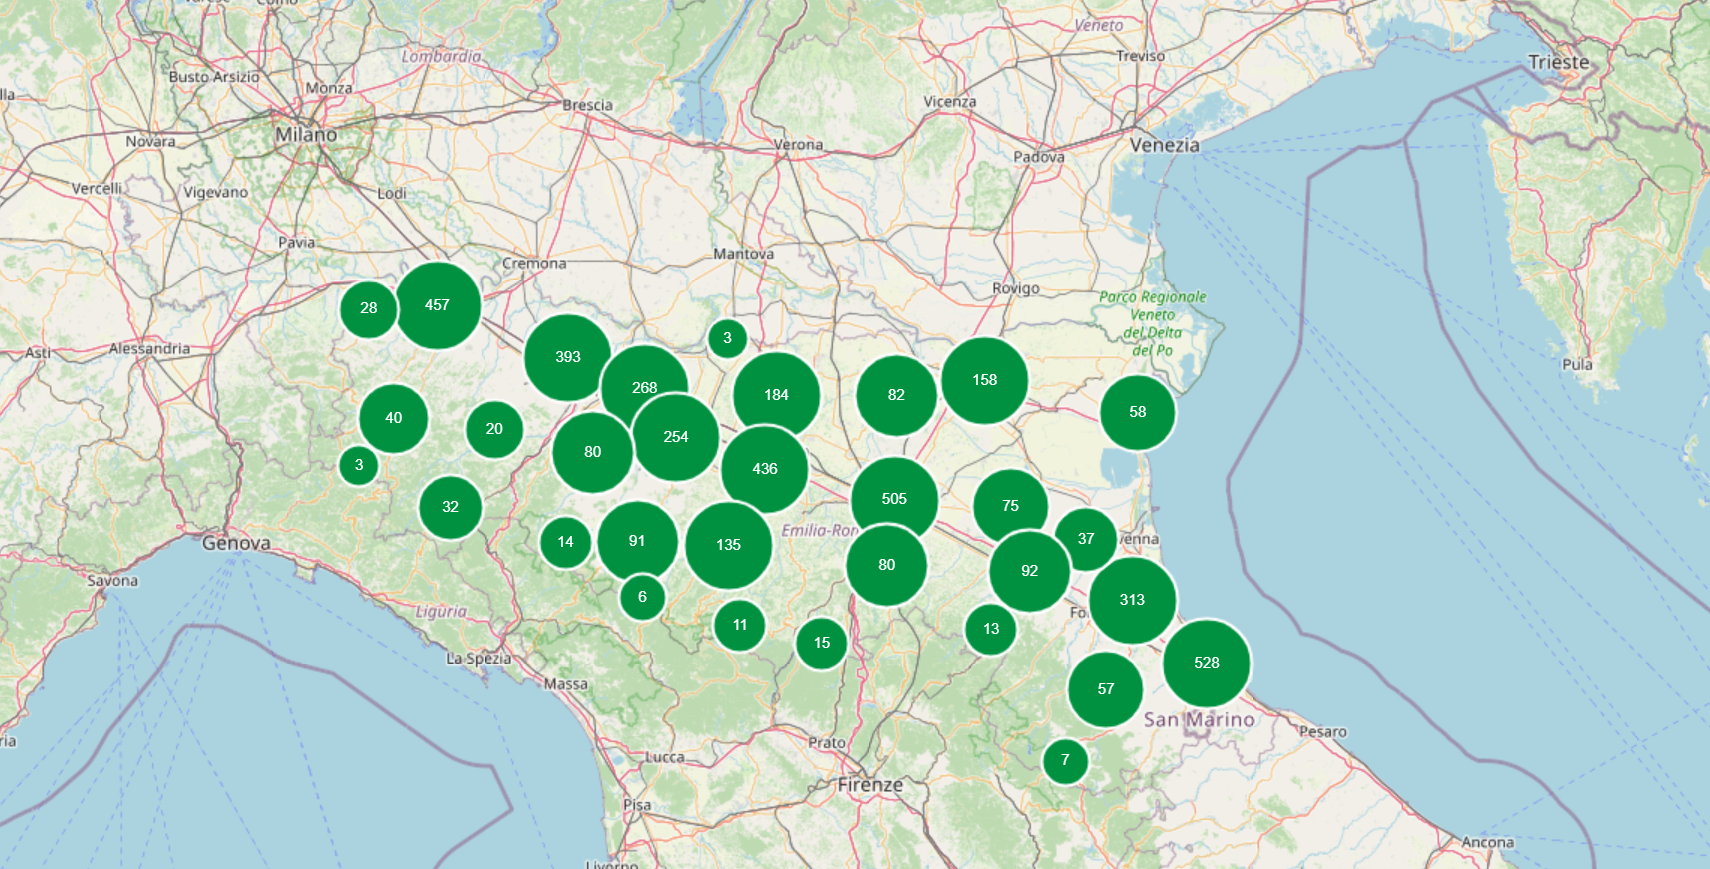
\includegraphics[width=\textwidth]{images/map.png}
    \caption{List of AEDs present in the region}
    \label{fig:DAE-map}
\end{figure}

Another prevailing function carried out by the software regards the implementation of a network of First Responders who, after the attainment of a qualifying certificate for the use of a defibrillator, enroll themselves in the register of the BLSD trained individuals and agree to intervene in case of a medical emergency.

Joining the project is entirely voluntary and does not imply obligations of any kind.
%
Registration can be done directly through the application, but we will see later on all the details regarding the registration process and requirements.

\subsection{Purpose of the Project}
Sudden cardiac arrest is a leading cause of death in Italy, with over 150,000 victims every year.
%
During a cardiac arrest, the victim's heart has an abnormal heart rhythm called ventricular fibrillation, which causes a loss of functionality in the heart that stops blood pumping to the rest of the body.

For the victim of cardiac arrest, every minute that passes matters: in sixty seconds  his chances of survival are lowered by 10\%. After only 5 minutes, the chances of salvation drop to 50\%.

From the moment in which breathing and blood circulation stops, the body tissues no longer receive oxygen, which is an element of fundamental importance for their survival. 
%
Once this process begins, the chances of surviving as well as the chances of a possible recovery in the absence of damage, especially in the brain, decrease considerably.

On the contrary, by intervening in a timely manner with a few simple first aid maneuvers, the chances of survival, as well as the possibility of recovery without brain damage, increase considerably.
%
Defibrillation is the only therapy to trait someone in cardiac arrest and represents one of the key steps in saving a life from sudden cardiac arrest.

The HeartBeat project aims at facilitating rapid intervention from trained individuals while waiting for the ambulance to arrive. 
%
Moreover, it allows first responders to identify the closest AED so that they can carry out rapid defibrillation and maximize the victim's survival chances.

\subsection{Scope of Work}
The software is designed as an extension of the management software used by the 118 Emergency Communications Centers, as it is fully integrated with its technologies.

The software used by the Emergency Communications Center allows 118 operators to follow each step related to an emergency request, allowing them to manage the following types of services:

\begin{itemize}
    \item Emergency / Urgent Transport
    \item Secondary Transport
    \item Transport by Helicopter Rescue
\end{itemize}

The Emergency Communications Center makes use of advanced technological solutions that guarantee the security of call reception systems, the user's exact location and real-time control of the position of the available emergency vehicles. 

They have a dedicated radio and telephone communication system which coordinates rescue interventions and guarantees the interoperability of Emergency Centers at an inter-regional level in case of catastrophes and maxi-emergencies.
%
The management and organization of the service can be of regional competence, provincial or delegated to individual Local Health Authorities (like AUSL).
%
The region of Emilia Romagna has 3 Communications Centers, each of which has an advanced telecommunication system for receiving and sorting all requests.
%
The personnel operating at the 118 Communications Center is made up of Professional Nurses suitably trained to be able to manage the complexity of the system.

\subsubsection{The Current Situation}
In case of medical emergency, once the request has been accepted and understood, the nurse of the Emergency Communications Center chooses the most suitable rescue resource in the area to entrust the service. 
%
The crew of the identified rescue vehicle receives the address, the patient's name and a code (which combines the priority code and other data such as the type of intervention and the geographical area), the time and a service identification number.

This procedure foresees the localization of the event and an immediate evaluation of the urgency level of the call. 
%
The staff at the time of answering: 

\begin{enumerate}
    \item Locates the event, using a dedicated management software equipped with an advanced cartographic module;
    \item Evaluates the severity of the event and assigns a priority to the request with a color code;
    \item Sends an emergency vehicle that is suitable for the emergency;
    \item Coordinates the development of the rescue intervention, identifying hospital facilities that are suitable for the rescued patients;
\end{enumerate}

Once on site, the personnel sent proceeds to assess the injured person and, after the stabilization and first aid maneuvers, contact the communications center to transmit the patient's data, the situation encountered and to obtain information regarding the hospital to which possibly go.

\subsubsection{External Entities}
The diagram showed in figure \ref{fig:context} outlines how external entities interact with the software system.

\begin{figure}
    \centering
    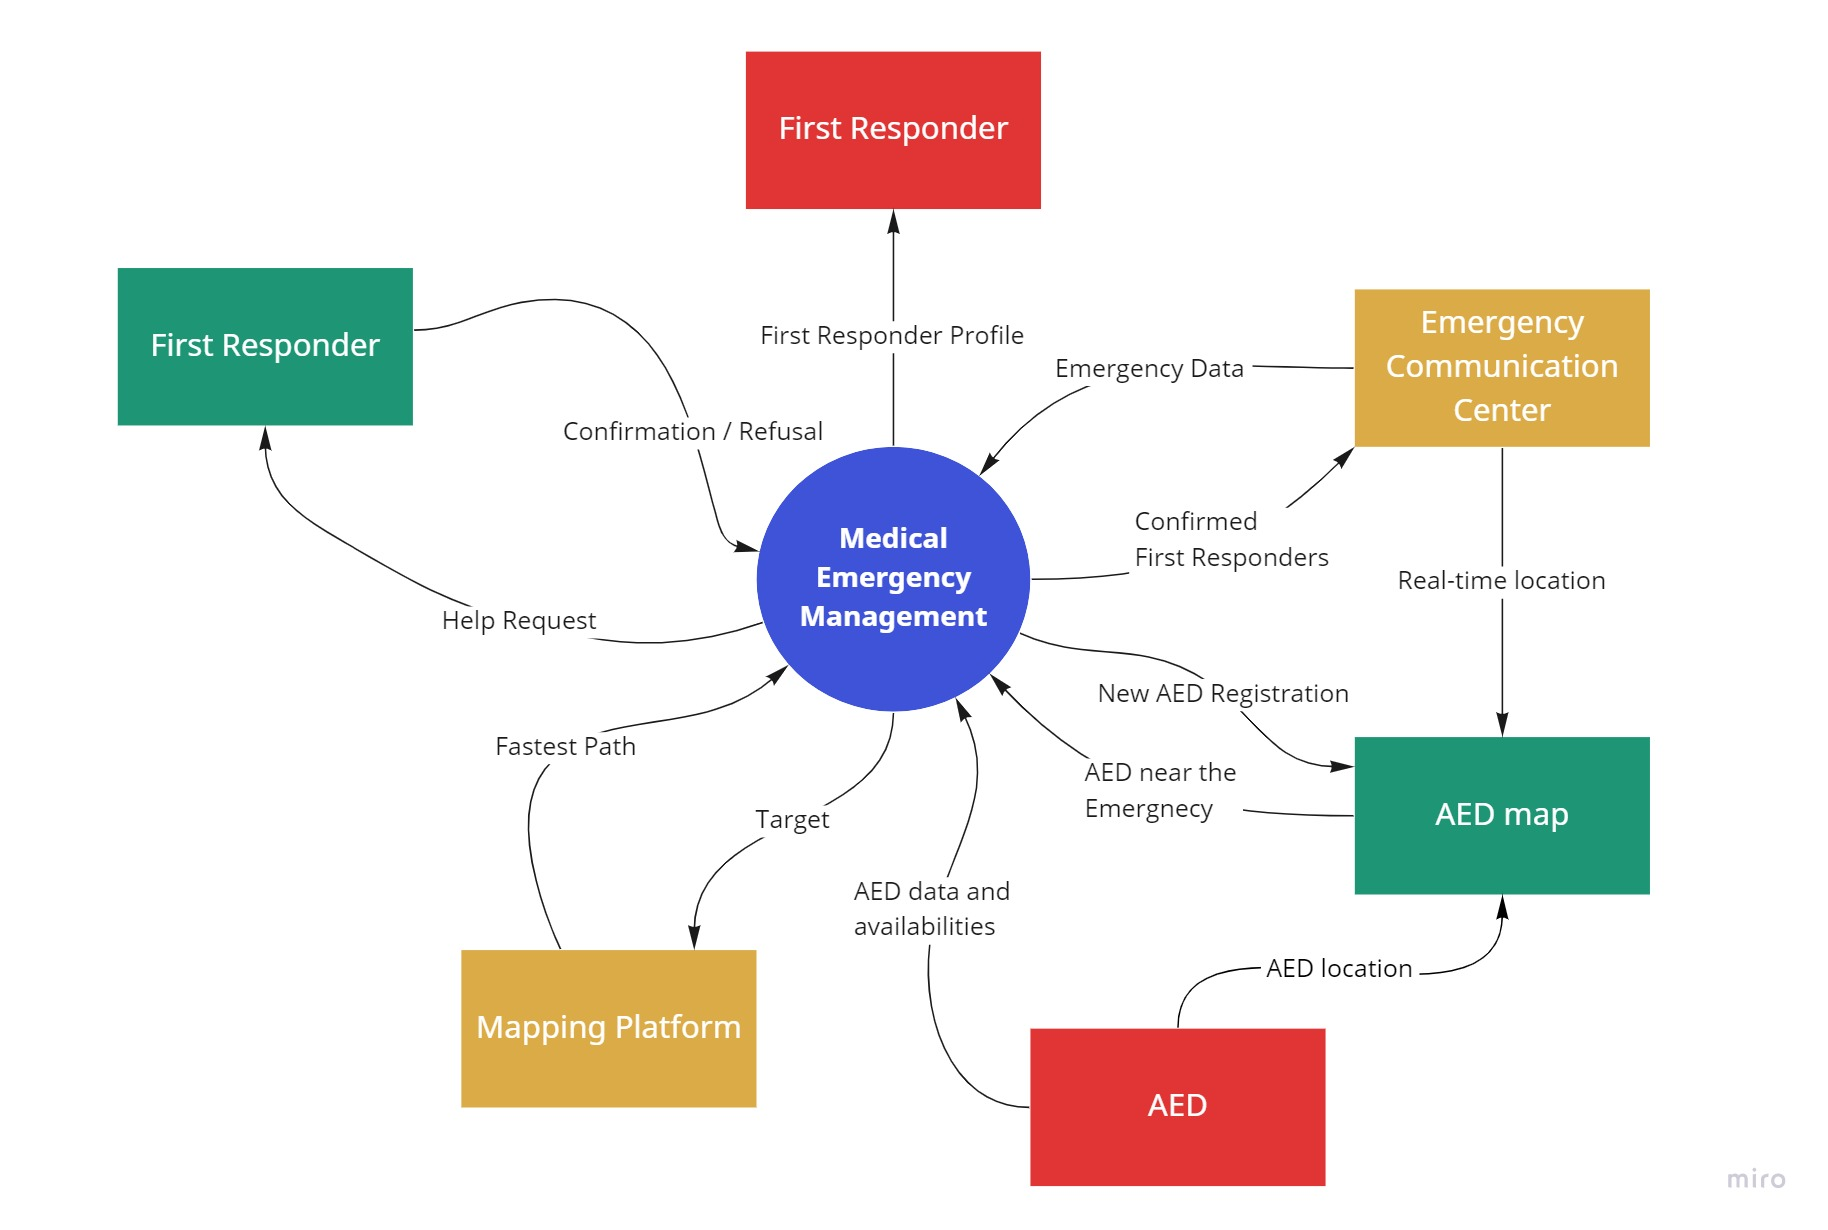
\includegraphics[width=\textwidth]{images/context.jpg}
    \caption{Component Diagram showing External and Internal Entities}
    \label{fig:context}
\end{figure}

The main entity with which the software interacts is the Emergency Communication Center, due to its central role in the emergency management process:
%
First of all, the request alert sent to first responders located in the area of interest is triggered by the assignment of the 'code blue' to the emergency.
%
This code indicates that the patient has compromised vital functions in an out-of-hospital environment and is assigned in case of cardiac or respiratory arrest.

Then, the local distribution of publicly available AEDs is connected with the 118 cartographic system and, at the same time, the registration of new AEDs carried out through the application also updates the system. 
%
During the emergency, the application not only displays the AEDs located in the area of interest, but it also provides information about their availability (if the defibrillator is located inside a shop that is closed at the time of the event, the first responder will not be able to reach it).

Next, the professional who handles the emergency call will see in real-time the first responders who accepted the help request and their movements on the map.
%
In this way, rescuers will have precise data about the time of intervention, which constitutes relevant details about the patient's conditions to be communicated to healthcare professionals.

Finally, another important interaction between entities regards the calculation of the fastest path to follow to reach the emergency location. 
%
This will be in charge of the mapping software which is already installed in the device (either google maps, apple maps and others).
%
The exact location of the emergency, initially provided by the Emergency Communications Center, will be displayed on the application and the path to follow to reach either the closest AED or the emergency target will be calculated by the mapping platform.

\subsection{Stakeholders and Actors}
The HeartBeat project is not designed for a specific market share, but it concerns the well-being of the entire territorial community. 
%
First responders represent the core identity of the software, so users can be considered as the main actors of the software system. 

We can identify two main macro-categories of users, which are not mutually exclusive:
On one hand, people who obtained a qualifying certificate for the use of a defibrillator - and therefore know the maneuvers to implement in the event of cardiac arrest - belong to the network of first responders.

On the other hand, business owners who install an AED in the building and register it through the application, have a fundamental role in implementing the network of publicly available defibrillators.
%
As we said before, being part of one category does not exclude the other one: a user who registers a new AED and is trained to use it, is also a first responder.

\section{System Use Cases}
To identify the domain events that are relevant for the design of the system, we applied the event-storming technique (showed in figure \ref{fig:event}) during which we walked through the model forwards and backwards to ensure that everything was covered.

We started by collecting all the events of interest, which we progressively ordered following their logical sequence.
%
Then, we modeled the process by exploring the commands and triggers that cause the events together with the sources of such commands, including users and external systems.
%
Finally, we identified aggregates and grouped them together into bounded contexts.
%
Along the way, key test scenarios, users, and goals were identified and incorporated into the model. 

\begin{figure}
    \centering
    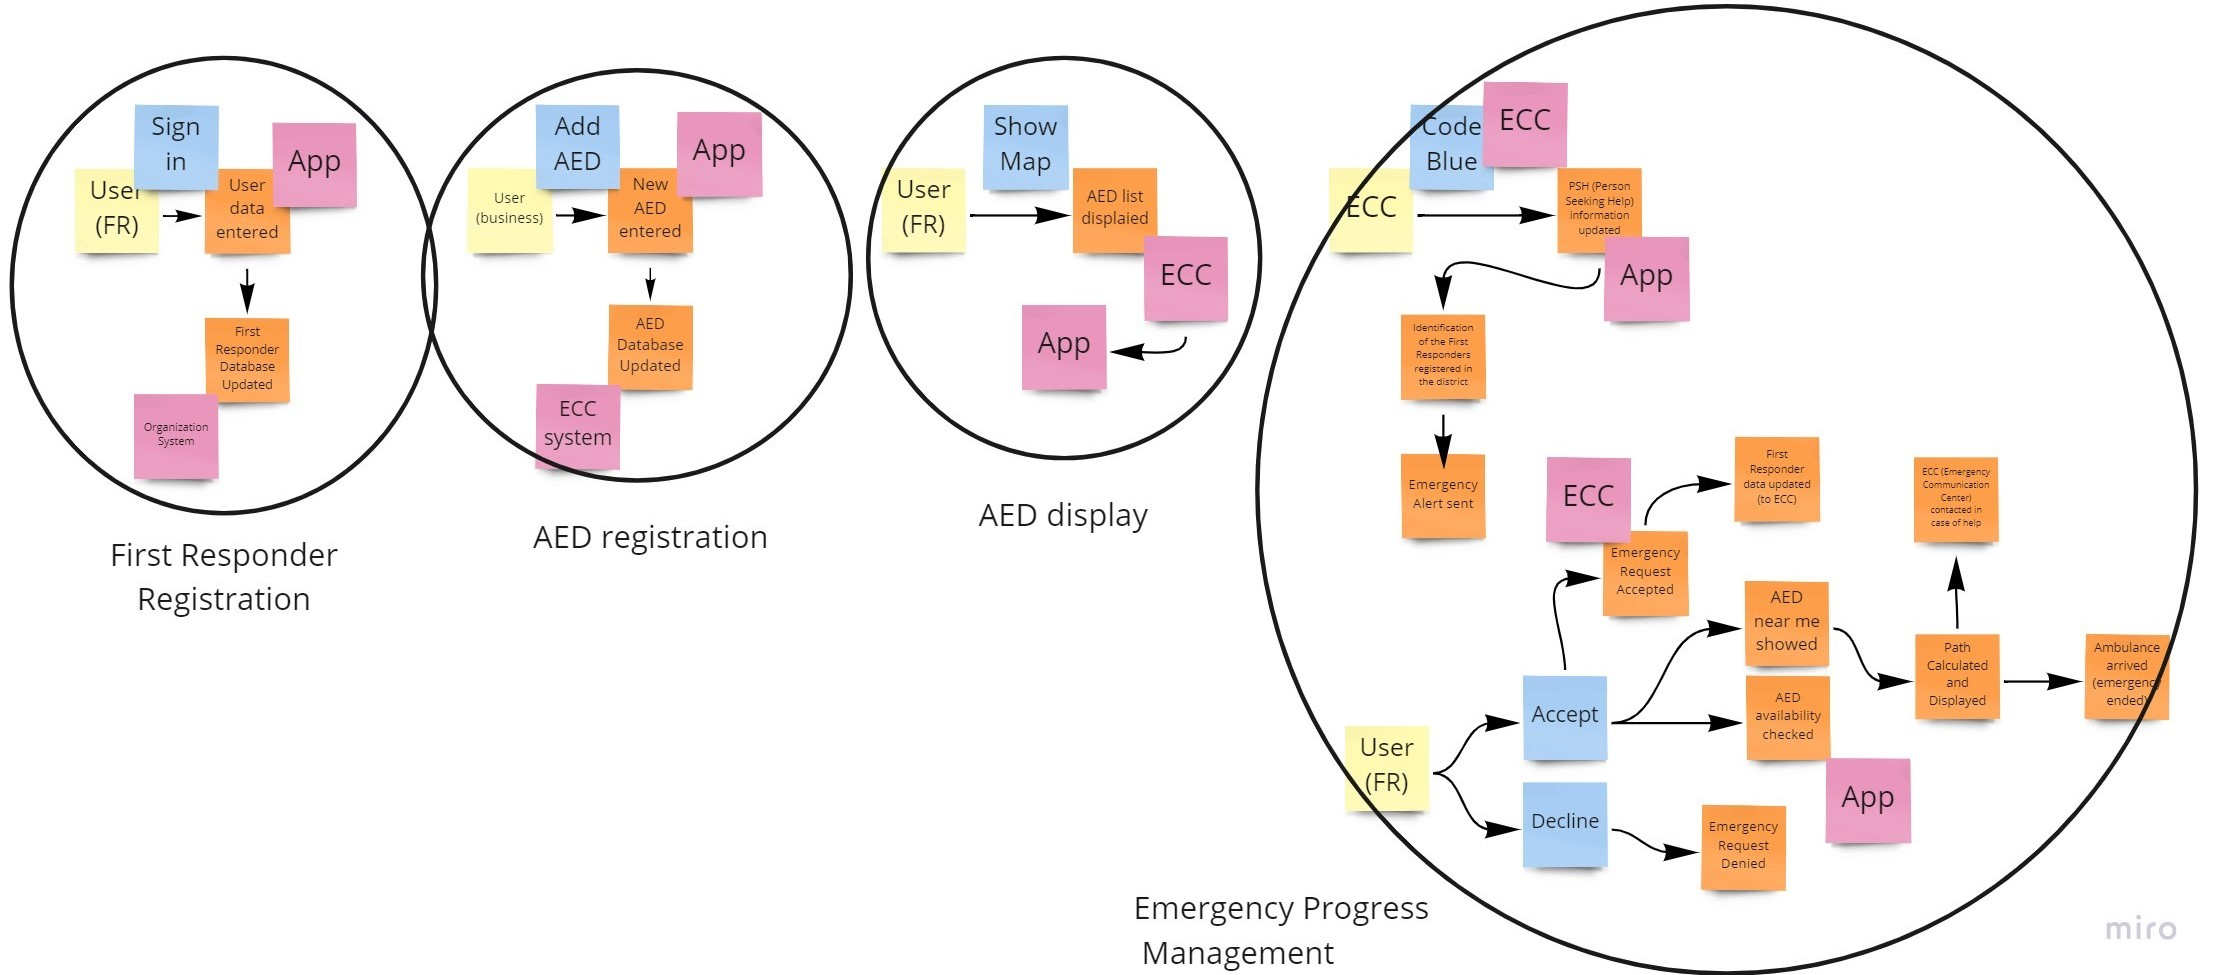
\includegraphics[width=\textwidth]{images/event-storming.jpg}
    \caption{Event-Storming with Aggregates and Bounded Contexts}
    \label{fig:event}
\end{figure}

\subsection{Analysis of Subdomains}
In this section we will describe in more specific and precise detail the steps that the system takes in the course of its functioning.
%
After the event-storming phase, three main basic subdomains have been identified:

\begin{enumerate}
    \item Emergency Progress Management (\textit{core})
    \item User Account Management (\textit{generic})
    \item AED Database Management (\textit{supporting})
\end{enumerate}

To facilitate our understanding, we decomposed the domain into subdomains. 
%
In this way, we are able to separate what in fact generates value, and thus, we can analyze more in dept all the aspects of the specific subdomains.

We identified the Emergency Progress Management as the core subdomain as it represents the activity that is uniquely performed by the system.
%
This domain is so critical and fundamental to the business that it generates a competitive advantage and is a foundational concept behind the business.

Then, the User Account Management constitutes the generic subdomain as it does not generate competitive advantage and it does not distinguish the system in the market.

Although this is a critical business concept, it is not core to the system and it can be outsourced and then wrapped in such a way to communicate with the rest of the system as necessary.

And finally, the AED Database Management supports the system in performing its main functions.

\subsubsection{Use Case Analysis}

\begin{figure}
    \centering
    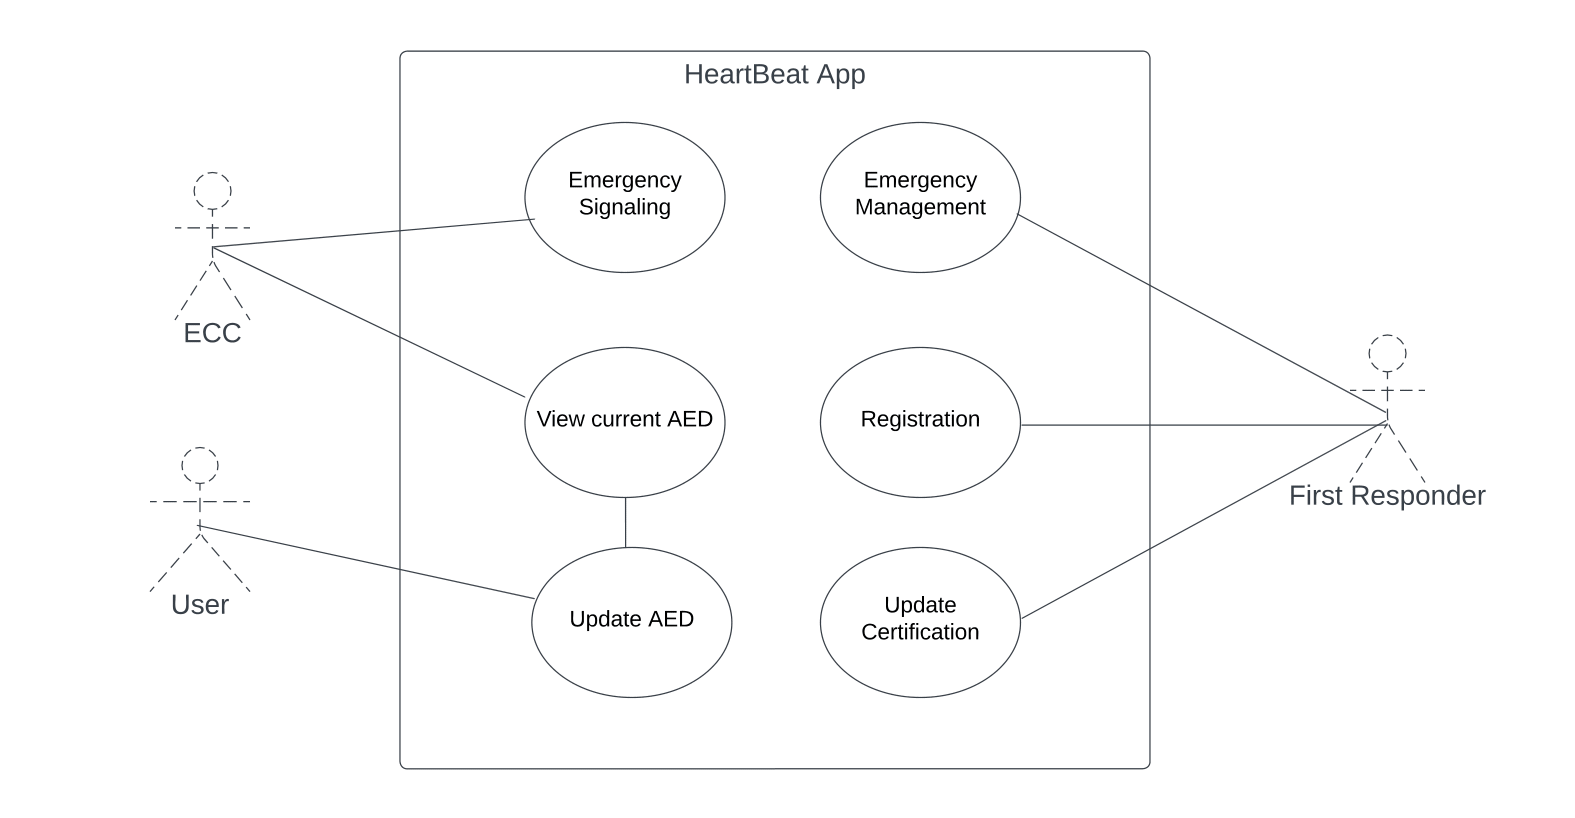
\includegraphics[scale=0.7, width=\textwidth]{images/use-case.png}
    \caption{Use cases Diagram}
    \label{fig:uml-emergency}
\end{figure}

In this section, we will analyze more in details each use case identified in the HeartBeat system, identifying all the key steps performed.

As we can see in figure \ref{fig:uml-emergency}, three actors are involved in the system functioning: 
%
The Emergency Communication System, First Responders and users.
%
Each actor performs specific actions based on the specific use case that takes place.

\subsubsection*{Emergency Signalling}

\begin{itemize}
    \item Primary actor: Emergency Communication Center
    \item Scope: Send the emergency alert to First Responders
    \item Scenario: Somebody calls the 118 for a medical emergency regarding a cardiac arrest
\end{itemize}

It all starts when the '118' emergency number is called for a victim of cardio-respiratory arrest.
%
As soon as the operator has verified that the emergency regards a cardio-respiratory arrest, he/she assigns the \textit{code blue} to it.
%
The assignment of the \textit{code blue} to an emergency triggers the \textbf{emergency management system}, which receives the data about the emergency and starts searching for suitable First Responders.

 First responders are selected according to two variables:

 \begin{enumerate}
     \item If the geo-location on the mobile phone is active, First Responder located within 1 km from the emergency site, will be notified.
     \item If the geo-location on the mobile phone if switched off, First Responders will be notified according to the municipality selected during the registration.
 \end{enumerate}

This use case terminates when suitable First Responders receive the \textbf{emergency alert}.

\subsubsection*{View Current AED}

\begin{itemize}
    \item Primary actor: Emergency Communication Center and Users / First Responders
    \item Scope: Visualize AEDs on the map and display information
    \item Scenario: Users want to see AEDs located near them in a specific moment
\end{itemize}

When a user wants to see AEDs displayed on the map, the system will detect the device location,and will display AEDs located in the area of 1 km from the user.

The distance of 1km is set as default but users can zoom in/out the map to limit/extend the research.
%
In the case in which the users' location is not available, the system will display AEDs according to the municipality selected at the time registration.

Each AED stored in the database has a profile containing all the relevant information, including the address, the reference point and available hours.
%
Once the user selects a specific defibrillator, the system will display these data.

\subsubsection*{Update AED}

\begin{itemize}
    \item Primary actor: Emergency Communication Center and Users / First Responders
    \item Scope: New AED is inserted in the system
    \item Scenario: A new AED is inserted in the system by the Emergency Communication System or a user
\end{itemize}

When a user or the Emergency Communication System wants to register a new AED, he/she will need to fill out the registration form with the following data:

\begin{itemize}
    \item Name of the place (reference point)
    \item Address
    \item Location (coordinates)
    \item Additional information about the location [optional]
    \item Availability (month - days - hours)
    \item Picture [optional]
\end{itemize}

Then, once the form has been submitted, the system confirms the registration of the new AED and updates the ECC database with the new information.

\textit{Extension}: Registration may fail due to invalid or missing data. If this happens, the user will have to re-enter the data and wait for confirmation.

\subsubsection*{Emergency Management}

\begin{itemize}
    \item Primary actor: First Responders
    \item Scope: Accept / decline the emergency alert
    \item Scenario: A First Responders receives an emergency alert and either accepts or declines it
\end{itemize}

When a first responder receives a help request, he/she clicks on the notification, which will automatically open the application and turn the geo-location on.

The First Responder can accept, decline or ignore the alert.
%
Once the First Responders has accepted the request, the system will send a confirmation to the Emergency Communications Center, which will see the responder's movements in real-time.

At the same time, the system will display the emergency details to the first responders who accepted the request, which are respectively:

\begin{itemize}
    \item Time of alert
    \item Reference point
    \item Address
    \item Ambulance ETA
\end{itemize}

\subsubsection*{Registration}

\begin{itemize}
    \item Primary actor: First Responders
    \item Scope: New users join the application
    \item Scenario: A user that has obtained a BLSD certificate wants to subscribe to the application creating their profile
\end{itemize}

After having downloaded the application, users will fill a registration form with the following data:

\begin{itemize}
    \item Name and Surname
    \item Email [to be confirmed]
    \item Municipality (if the geo-localization is not active, the emergency alert will be sent according to the municipality selected) 
    \item BLSD certificate (emission body)
    \begin{itemize}
        \item Date of emission
        \item Period of validity
    \end{itemize}
    \item Tax code
    \item Picture [optional]
\end{itemize}

At the time of registration, users will also have to authorize the access to location (when using the app), as well as confirm the terms and conditions of the application.
%
Once users have submitted the form, they will wait for confirmation to be sent by the system.

\textit{Extension}: Registration may fail due to invalid or missing data. If this happens, the user will have to re-enter the data and wait for confirmation.

\subsubsection*{Update Certificate}

\begin{itemize}
    \item Primary actor: First Responders
    \item Scope: Update an expired certificate in order to be able to intervene in case of emergency
    \item Scenario: The BLSD certificate will expire within a one-month period
\end{itemize}

The system will automatically calculate the date of expiry and, one month before, it will notify the user to update the certificate.
%
Users can update their certificate at any time by updating their profile.

\textit{Extension}: Updating may fail due to invalid or missing data. If this happens, the user will have to re-enter the data and wait for confirmation.

\section{Software Requirements}
In this section we will describe the features and functionalities that users expect from the software.

Through requirements specification, we defined how the software should interact with external interfaces, the speed of operations, the response time of the system, the portability of the software, maintainability, security and others.

\subsection{Performance Requirements}
Performance requirements define how well the software system accomplishes certain functions under specific conditions.
%
To assess the performance of the system, we analyzed the following characteristics: response time, workload and scalability.

The response time refers to the time employed to execute and complete specific tasks. 
%
Considering the environment in which HeartBeat operates, speed of execution is a crucial aspect:

The goal of the software is to minimize the time of intervention in case of cardiac arrest, so, it is essential for the micro-services to communicate rapidly with each others and with the user app.

To assess the workload, we built a table of volumes to estimate data volumes and usage frequency of the databases of the system.
%
In table \ref{table:volume}, we estimated the volume of data flowing to the database systems, in the region of Emilia Romagna, every month.

\begin{table}
\centering
\begin{tabular}{|c c c|} 
 \hline
 Concept & Typology & Volume \\ [0.5ex] 
 \hline\hline
 User Data & Static & 150 \\ 
 AED & Static & 50 \\
 Emergency Data & Static & 600 \\
 Real-time Location & Dynamic & 300 \\
 First Responder & Dynamic & 300 \\ [1ex] 
 \hline
\end{tabular}
\caption{Data Volumes and Frequency}
\label{table:volume}
\end{table}

As we can see, around 150 new users download the application and enroll themselves to the register of first responders.\footnote{DAE responER application reached 10.000 users  in 4 years, with an average of 200 new users each month. [https://www.118er.it/dae/news]}

Then, we estimated around 50 new AEDs added each month to the regional register of defibrillators, which would imply updating both the ECC official list and the HeartBeat database.

Emergency data refers to the data that are shared by the Emergency Communications Center every time a 'code blue' is recorded.
%
Keeping in mind that around 150.000 people are victim of sudden heart attack every year, we estimated around 600 emergencies in the area of Emilia Romagna every month.

Finally, first responder refers to the recording of the data of users who accepted the emergency alert, while real-time location concerns the recording of their coordinates.
%
The frequency of these two entities is the same and we estimated that given 600 sudden cardiac arrest, HeartBeat would successfully identify suitable first responders and AED 50\% of the times.

Scalability refers to the ability of the software to handle increased workloads with minimal cost impact.
%
In this case, keeping in mind that HeartBeat operates on a regional level, data should flow at a constant rate.

Of course, in case of expansion, the system would have to deal with increased workload and scalability issues.
%
However, for what concerns performance requirements, the most important one regards the speed of execution.

\subsection{Dependability Requirements}
The dependability of a system reflects the user's degree of trust in that system. 
%
It reflects the extent of the user's confidence that it will operate as users expect and that it will not 'fail' in normal use. 

Dependability covers the related systems attributes of availability, reliability, security, integrity and maintainability.

\subsubsection{Availability}
Availability refers to the percentage of time that the infrastructure, system, or solution remains operational under normal circumstances in order to serve its intended purpose. 

For HeartBeat, availability is a key aspect as sudden cardiac arrests are unpredictable and can happen any time.
%
This is the reason why the system must be always running properly; a service downtime could lead to tragic outcomes.

\subsubsection{Reliability}
Reliability refers to the probability that the system will meet certain performance standards in yielding correct output for a desired time duration.

Also here, it is important for the system to keep running accurately in time, minimizing failures and delivering services as expected by users.
%
For example, in the event of an emergency, users expect the data about the AED location to be precise and accurately displayed through the mapping system.

At the same time, it is important for the Emergency Communications Center to receive real-time movements of first responders to collect relevant information about the time of intervention.

\subsubsection{Security}
Software security is the concept of implementing mechanisms in the construction of security to help it remain functional (or resistant) to attacks. 

This means that a piece of software undergoes software security testing before going to market to check its ability to withstand malicious attacks.

Security is a key aspect for HeartBeat as it is important to prevent attacks that jeopardize systems' availability and reliability.
%
Moreover, the system deals with sensitive information which must be protected from potential attackers.

\subsubsection{Integrity}
With system integrity, we include the attributes that we have analyzed so far.
%
Software integrity refers to the quality of the software’s source code, which is essentially a measure of how safe, secure, and reliable it is.

Code quality is directly related to higher security and protection against threats, but also to the maintainability and testability of the code. 

All of these factors play an important role in the software development, and ultimately contribute to the implementation of a better system. 

\subsubsection{Maintainability}
Maintainability represents the degree of effectiveness and efficiency with which a product or system can be modified by the intended maintainers. 

The Maintainability of an application is a combination of compliance with good coding practices, the homogeneity with which coding rules are applied across an application, and compliance with architectural rules.

Since software is not static, the ability of a software to evolve and change is of key importance in today's agile environment.

\section{Project Design and Development}
Software design is the process of envisioning and defining software solutions to one or more sets of problems.
%
To do so, we followed some key design principles like abstraction, modularity, data structure and software procedure.

To retain only relevant information, we included only essential features without including background details.

Then, we divided the architecture into components, developed individually, keeping an eye on the overall structure.

And finally, we tried to represent the logical relationship among individual elements of data.

\subsection{Software Architecture}
Software architecture is, simply, the organization of the system. 

This organization includes all components, how they interact with each other, the environment in which they operate, and the principles used to design the software.

We can classify all these elements into three categories:

\begin{enumerate}
    \item Database System
    \item Front-end Technologies
    \item Back-end Technologies
\end{enumerate}

In this section we will explore each micro-service that composes the system, focusing on the relationships among the components and analyzing how they interact with each other.

\subsection{Database System}
In our project, the implementation of multiple databases is essential to collect and manage data in a systematic way.

First, all the information regarding users must be stored and updated in case of changes. 
%
Users' data, identified by a user ID, will be automatically accessed by the system through SQL queries as soon as they are needed for the emergency progress system. 

Then, the registered AEDs must be stored indicating the precise location (expressed using geographical coordinates), the name of the place and all the information regarding their availability.

Finally, data about the emergency will be stored in a database that is connected to the emergency micro-service.
%
The system will attribute an ID to each emergency and will store the following data:

\begin{itemize}
    \item Coordinates of the emergency.
    \item List of first responders who received the alert (specifying whether they have accepted or declined it).
    \item List of AEDs located near the emergency.
\end{itemize}

\subsection{Back-End Development}
The back-end refers to the parts of the application that allow it to operate and that cannot be accessed by users.
%
We identified three micro-services that communicate with each other and with the mobile application through REST APIs.

The first micro-service regards all the operations concerning users' accounts.
%
More in details, the tasks performed by the account-service include:

\begin{enumerate}
    \item Communication with the accounts' database through SQL queries to insert, update and delete accounts.
    \item Identification of the suitable first responders on the basis of the location of the emergency.
    \item Creation and management of the notification alerts sent to users.
\end{enumerate}

Then, the operations regarding AEDs locations are in charge of the AED-service. 
%
In particular, the tasks performed by this micro-service include:

\begin{enumerate}
    \item Communication with the AED database through SQL queries to insert, update and delete AEDs.
    \item Identification of the AEDs located near the emergency.
    \item Display of AEDs on the user app.
\end{enumerate}

In listing \ref{lst:api}, the design of the APIs that allow the communication between these two micro-services is displayed.
%
Here we can see some examples of 'get' and 'post' requests on users' accounts, as well as some 'get' requests on the AED-service.

In the first example, the system will essentially display the text "This is an API between users and AED locations", showing that the system is running on the selected port.

Then, app.get('/users') returns the list of users stored in the database and, through the function 'convertToUserDto', it only displays the userId, name and city of each user. \\

\lstinputlisting[language=JavaScript, label=lst:api, caption=API design between account-service and AED-service]{listings/API.js}

Moving to AED locations, app.get('/locations') simply returns the list of the AEDs present in the database, displaying the name of the place in which they are located and the identification number of each defibrillator.

Here below we can see the output of the locations get request, which is characterized by a JSON file specifying data for each registered AED.

The last http method displayed simulates the behaviour of the system in the moment in which, given a location, the account micro-service identifies the users that are located in the area. \\

\begin{lstlisting}[language=JSON]
[
    {
        "locationid": "0001",
        "name": "Cesena Train Station"
    },
    {
        "locationid": "0002",
        "name": "Ravenna Sports Center"
    },
    {
        "locationid": "0003",
        "name": "Bologna Train Station"
    },
                .
                .
                .
    {
        "locationid": "0014",
        "name": "Rimini University Campus"
    }
]
\end{lstlisting}

For example, figure \ref{fig:get} shows a get request held between the account-service and AED-service, in which the latter gives as input the id of a specific defibrillator - which in the example corresponds to locationId = 0007, the Cesena University Campus - and the former returns data about the users who are located nearby.

\begin{figure}
    \centering
    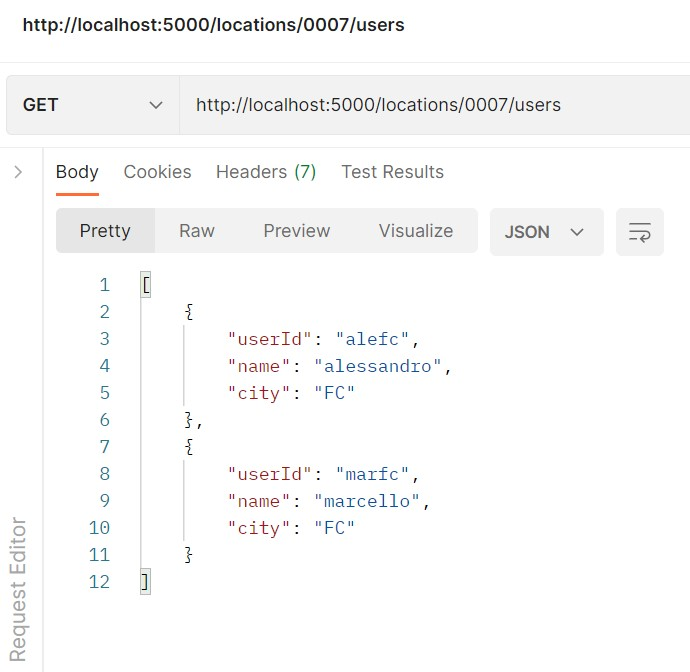
\includegraphics[height=9cm, width=10cm]{images/get-api.jpg}
    \caption{Get request showing users that are located near AED n°0007}
    \label{fig:get}
\end{figure}

The last micro-service that is part of the back-end development is the emergency-service.
%
This service communicates with the other two services through REST APIs, as we saw in the example above, and with the emergency database through SQL queries.
%
The tasks performed by the emergency-service, include:

\begin{enumerate}
    \item Elaboration of the data received by the Emergency Communications Center and emergency database update.
    \item Sharing of the emergency data to the other micro-services and the user app.
    \item Sharing with the Emergency Communications Center of the data about first responders who accepted the alert.
\end{enumerate}

\subsection{Front-End Development}
Front-end development refers to the client side of the system with which users can interact directly.
%
For HeartBeat, users have at disposal both a mobile app and a web portal:

The mobile app represents the main interface for users as some operations need direct access to active localization, camera or the calling system.
%
While the web portal only constitutes an alternative means by which users can update their profiles.

The user app communicates with the micro-services through REST APIs in order to transfer data from users to services and vice versa.
%
In particular, its tasks include:

\begin{enumerate}
    \item Users' data entry and update.
    \item AEDs' data entry and update.
    \item Display of the notification alert and sharing of the data of users who accept it.
    \item Display of AEDs and communication with the mapping platform.
\end{enumerate}

\section{Conclusions}
Working on this project proved to be a great challenge for us, especially because of our non-technical academic background.
%
We found it difficult to remain coherent along all the process of design and trying to integrate all the notions from the course was not easy.

During the planning phase, we found it very useful to conduct an event storming session, which allowed us to develop a common knowledge and understanding of the business domain.

Along the way, we encountered some difficulties related to the business domain specifically but fortunately, we could rely on the opinion of some domain experts who work in the emergency sector.
%
Indeed, we were able to take some relevant decisions about the design of the system thanks to their expertise.

Also, tracking the project using GitHub was quite hard initially as we approached it at a technical level for the first time.
%
On the other hand, we had the possibility to explore the potential of GitHub to store, manage and track projects, both developed individually and in team.

Overall, we agree on the added value that this project gave us, allowing us to see in practice the importance of the techniques studied during the course, by applying them in a real world scenario.

\subsection{Domain Driven Design}
Concerning the Domain Driven Design, we started with a long planning session in which we tried to pin down all the concepts to have a clear holistic view of the whole system.
%
After having identified the domain, we were able to map the context of work, identifying all the entities involved in the system.

The design of bounded contexts was identified as the most challenging aspect of DDD, whilst the analysis process carried out with the tools and the philosophy transmitted during the course felt quite natural and effective since the beginning.

Furthermore, developing a ubiquitous language for the project turned out to be extremely useful to align the team and provide a common understanding.

\subsection{DevOps}
DevOps is a set of practices which aims at shortening the systems' deployment life cycle by providing continuous delivery and high software quality.

Together with iterative software development, automation, and programmable infrastructure deployment, DevOps also covers culture changes, such as building cohesion between developers and administrators and aligning technological projects to business requirements.

To implement DevOps in our project, the first step to undertake regards the effective integration of people, processes, and tools to obtain a single entity.
%
The purpose is to encourage collaboration and align IT goals with business strategy.

Then, it is essential to adopt an end-user-centric  process to deliver a service that exceeds users' expectations regarding time, functionality, and performance.
%
In this regard, DevOps aims at achieving efficiency by leveraging end-users feedback for constant improvement.

A key practice used in DevOps is automation: through automation, it is possible to save valuable resources in terms of cost, time, and efforts of developers and testers.
%
Continuous integration is the key to a successful DevOps strategy.
%
It enables developers to build software in small, regular steps by immediately identifying defects and rendering feedback.

\subsection{Future Improvements}
After having discussed in group about potential future improvements, we identified two features that could enhance the user experience:

\begin{itemize}
    \item Gamification.
    \item Emergency Progress Status.
\end{itemize}

Gamification refers to the application of game-design elements, in non-gaming contexts, to educate, entertain and engage users.
%
Here, the idea would be to introduce gamification elements to stimulate learning and training experiences towards health, first aid and emergencies' management.

The Emergency Progress Status, on the other hand, regards an additional feature which allows first responders receiving the help request to see the status of the emergency.
%
More in details, they would be able to see the number of people who accept the request, their movements in the map and they would have the possibility to contact them.

\section{Ubiquitous Language}

All project-related stakeholders, such as software engineers, domain experts and UI/UX designers, should use a single language for describing the business domain: the Ubiquitous Language. 

This approach consist of business domain related terms only and no technical jargon, so everyone can capture the main concept not on a technical level, but rather on a business level which is easily explainable. 

Regarding HeartBeat project, we have captured terms and concepts into a glossary to develop its Ubiquitous Language.

\subsection*{AED}
Automated External Defibrillator.
%
It is a portable electronic device that automatically diagnoses the life-threatening cardiac arrhythmia's of ventricular fibrillation and pulse-less ventricular tachycardia.
%
It is able to treat them through defibrillation, allowing the heart to re-establish an effective rhythm.

\subsection*{AED Availability}
List of AED that are located in public or private structures, which can be not available during the closing hours.

\subsection*{AED Database}
AEDs must be stored indicating the precise location (expressed using geographical coordinates), the name of the place and all the information regarding their availability.

\subsection*{Code Blue}
Code assigned to the emergency by the ECC operator indicating that the patient has compromised vital functions in an out-of-hospital environment (usually assigned in case of cardiac or respiratory arrest).

\subsection*{ECC}
Emergency Communications Center, it is a fundamental structure for the management of territorial emergencies and it answers every individual's request for help.

\subsection*{Emergency Alert}
A warning notification sent by the Emergency Communication Center.

\subsection*{Emergency Request}
It is the notification that is sent to all the devices of the first responders who are located in a determined area, which can be accepted or refused.

\subsection*{First Responder}
Person with specialized training who downloaded the application.

\subsection*{PSH}
Person Seeking Help, a person asking or receiving help due to a sudden heart attack.

\end{document}
